\documentclass[12pt,a4paper,openany]{memoir}

\usepackage[portuguese]{babel}
\usepackage[T1]{fontenc}

\usepackage{makeidx}
\usepackage{xspace}
\usepackage{graphicx,color,times}
\usepackage{fancyhdr}
\usepackage{amsmath}
\usepackage{latexsym}
\usepackage[printonlyused]{acronym}
\usepackage{float}
\usepackage{listings}
\usepackage{tocbibind}
\usepackage{natbib}
\usepackage{booktabs}
\usepackage{tabularx}
\usepackage{array}
\usepackage{subcaption}
\usepackage{enumitem}
\usepackage{xcolor}
\usepackage{hyperref}
\hypersetup{colorlinks=true,linkcolor=blue,urlcolor=blue,citecolor=blue,
  pdftitle={GenJazz -- Relatório Final IHC}}

\graphicspath{{./screenshots/}}

\setlength{\parskip}{3pt}
\setlength{\parindent}{0pt}

\pagestyle{fancy}
\renewcommand{\chaptermark}[1]{\markboth{#1}{}}
\renewcommand{\sectionmark}[1]{\markright{\thesection\ #1}}
\fancyhf{} \fancyhead[LE,RO]{\bfseries\thepage}
\fancyhead[LO]{\bfseries\rightmark}
\fancyhead[RE]{\bfseries\leftmark}
\renewcommand{\headrulewidth}{0.5pt}
\renewcommand{\footrulewidth}{0pt}
\setlength{\headheight}{15.6pt}
\setlength{\marginparsep}{0cm}
\setlength{\marginparwidth}{0cm}
\setlength{\marginparpush}{0cm}
\addtolength{\hoffset}{-1.0cm}
\addtolength{\oddsidemargin}{\evensidemargin}
\addtolength{\oddsidemargin}{0.5cm}
\addtolength{\evensidemargin}{-0.5cm}

\usepackage{fix-cm}
\usepackage{fourier}
\usepackage{lmodern}
\definecolor{ChapGrey}{rgb}{0.6,0.6,0.6}
\newcommand{\LargeFont}{
  \usefont{\encodingdefault}{\rmdefault}{b}{n}
  \fontsize{60}{80}\selectfont\color{ChapGrey}}
\makeatletter
\makechapterstyle{GreyNum}{
  \renewcommand{\chapnamefont}{\large\sffamily\bfseries\itshape}
  \renewcommand{\chapnumfont}{\LargeFont}
  \renewcommand{\chaptitlefont}{\Huge\sffamily\bfseries\itshape}
  \setlength{\beforechapskip}{0pt}
  \setlength{\midchapskip}{20pt}
  \setlength{\afterchapskip}{25pt}
  \renewcommand\chapterheadstart{\vspace*{\beforechapskip}}
  \renewcommand\printchaptername{
  \begin{tabular}{@{}c@{}}
    \chapnamefont \@chapapp\\}
    \renewcommand\chapternamenum{\noalign{\vskip 2ex}}
    \renewcommand\printchapternum{\chapnumfont\thechapter\par}
    \renewcommand\afterchapternum{
  \end{tabular}
  \par\nobreak\vskip\midchapskip}
  \renewcommand\printchapternonum{}
  \renewcommand\printchaptertitle[1]{{\chaptitlefont{##1}\par}}
  \renewcommand\afterchaptertitle{\par\nobreak\vskip \afterchapskip}
}
\makeatother
\chapterstyle{GreyNum}

\setcounter{tocdepth}{2}
\setsecnumdepth{subsection}
\renewcommand{\ttdefault}{lmtt}

\definecolor{dkgreen}{rgb}{0,0.6,0}
\definecolor{gray}{rgb}{0.5,0.5,0.5}
\definecolor{mauve}{rgb}{0.58,0,0.82}

\lstset{basicstyle=\footnotesize\ttfamily,frame=single,breaklines=true,
  keywordstyle=\color{blue},commentstyle=\color{dkgreen},
  stringstyle=\color{mauve},belowskip=0cm}

\renewcommand{\today}{\day \ifcase \month \or Janeiro\or Fevereiro\or Mar\c{c}o\or %
Abril\or Maio\or Junho\or Julho\or Agosto\or Setembro\or Outubro\or Novembro\or %
Dezembro\fi de \number \year}

\begin{document}


\thispagestyle{empty}
\setcounter{page}{-1}

\begin{center}
\begin{Huge}
\textbf{Universidade da Beira Interior}
\end{Huge}
\end{center}

\begin{center}
\begin{Huge}
Departamento de Informática
\end{Huge}
\end{center}

\vspace{0.07cm}
\begin{figure}[!htb]
\centering

\includegraphics[width=191pt]{ubi-fe-di.png}
\end{figure}

\vspace{0.5cm}
\begin{center}
\begin{Large}
\textbf{Interação Humana Com O Computador \\ --- \emph{GenJazz}}\\[0.3cm]
\textit{Gerador de Progressões Harmónicas de Jazz}\\[0.2cm]
\textit{Relatório Final}
\end{Large}
\end{center}

\vspace{0.5cm}
\begin{center}
\begin{large}
Elaborado por:
\end{large}
\end{center}

\vspace{0.2cm}
\begin{center}
\begin{large}
\textbf{Francisco Branco - 51829 \\ Francisco Bondoso - 53905 \\ Afonso Cardoso - 54046}
\end{large}
\end{center}

\vspace{0.5cm}
\begin{center}
\begin{large}
Docente:
\end{large}
\end{center}

\vspace{0.2cm}
\begin{center}
\begin{large}
\textbf{Professor Doutor Adriano Raposo}
\end{large}
\end{center}

\vspace{0.5cm}
\begin{center}
\begin{normalsize}
\today
\end{normalsize}
\end{center}

\clearpage

\frontmatter
\chapter*{Agradecimentos}
\label{chap:ack}

Ao docente da unidade curricular, pela disponibilidade e pelos comentários que foram ajudando a afinar as decisões de design ao longo do semestre.

Ao criador da API GenJazz, disponível publicamente, sem a qual grande parte do projeto não seria possível.

\clearpage
\tableofcontents
\clearpage
\chapter*{Acrónimos}
\label{chap:acro}

\begin{acronym}[WCAG]

  \acro{API}{\emph{Application Programming Interface}}
  \acro{IA}{Inteligência Artificial}
  \acro{CSS}{\emph{Cascading Style Sheets}}
  \acro{HTML}{\emph{HyperText Markup Language}}
  \acro{IHC}{Interação Humana Com O Computador}
  \acro{JS}{\emph{JavaScript}}
  \acro{JSON}{\emph{JavaScript Object Notation}}
  \acro{RGPD}{Regulamento Geral sobre a Proteção de Dados}
  \acro{SPA}{\emph{Single Page Application}}
  \acro{UBI}{Universidade da Beira Interior}
  \acro{UI}{\emph{User Interface}}
  \acro{UX}{\emph{User Experience}}
  \acro{WCAG}{\emph{Web Content Accessibility Guidelines}}

\end{acronym}

\clearpage

\mainmatter
\acresetall
\chapter{Introdução}
\label{chap:intro}

\section{Enquadramento e Motivação}
\label{sec:enquadramento}

Este relatório apresenta a segunda e última fase do projeto \textbf{GenJazz}, desenvolvido no âmbito da unidade curricular de \ac{IHC} do curso de Engenharia Informática da \ac{UBI}. O GenJazz é uma aplicação móvel que gera progressões harmónicas de jazz a partir de parâmetros configuráveis --- tonalidade, estrutura formal e tipo de modulação --- e permite ao utilizador ouvir o resultado, visualizá-lo numa grelha de compassos e guardá-lo numa biblioteca pessoal.

A ideia surgiu de um problema concreto: o jazz tem uma linguagem harmónica rica mas pouco acessível a quem está a aprender. Há livros e partituras, claro, mas faltam ferramentas interativas que permitam explorar essa linguagem de forma rápida e auditiva. O GenJazz tenta preencher esse espaço de forma simples e direta.

Na primeira fase foram definidos o conceito, as personas, os fluxos de navegação e o protótipo de baixa-média fidelidade. Nesta fase, o protótipo foi implementado como aplicação web funcional e melhorado com base nas heurísticas de Nielsen~\cite{nielsen1994} e em princípios de design inclusivo.

\section{Objetivos}
\label{sec:objetivos}

Os principais objetivos desta fase foram: implementar o protótipo da Parte~1 como aplicação web funcional; integrar a API GenJazz para geração de progressões e conversão para áudio; e adicionar funcionalidades de acessibilidade para utilizadores com deficiência de visão cromática que não tinham sido contempladas no protótipo original.

\section{Organização do Documento}
\label{sec:organizacao}

O documento está organizado da seguinte forma: o Capítulo~2 descreve a arquitetura do sistema; o Capítulo~3 é o manual do utilizador; o Capítulo~4 apresenta as decisões de design e acessibilidade; o Capítulo~5 detalha as alterações face ao protótipo da Parte~1; e o Capítulo~6 contém as conclusões e o que ficou por implementar. O Apêndice~A é a declaração de uso de IA.

\clearpage
\chapter{Arquitetura do Sistema}
\label{chap:arquitetura}

O GenJazz é uma \ac{SPA} construída com \textbf{React~18} e \textbf{Vite}, que apresenta a interface dentro de uma moldura de smartphone para deixar claro que a experiência foi pensada para mobile. A arquitetura segue um modelo cliente-servidor simples: toda a lógica de apresentação corre no browser do utilizador, e os dados musicais são fornecidos por uma API REST externa alojada em \texttt{genjazz-api.fly.dev}.

\section{Stack e Organização do Código}
\label{chap2:sec:stack}

A escolha do React deveu-se à sua abordagem declarativa e ao sistema de componentes, que tornam mais fácil gerir os vários estados possíveis de uma interface com tantos elementos dinâmicos. O Vite foi preferido ao Create React App simplesmente por ser mais rápido --- tempos de arranque e hot-reload visivelmente melhores durante o desenvolvimento.

O código está organizado em \texttt{src/screens/} para os ecrãs completos, \texttt{src/components/} para componentes reutilizáveis (como o \texttt{CircleOfFifths}, o \texttt{AudioPlayer} e o \texttt{MeasureGrid}), e \texttt{src/hooks/} para lógica partilhada.

\section{Gestão de Estado e Autenticação}
\label{chap2:sec:estado}

O estado global é gerido por dois contextos React. O \texttt{AuthContext} trata da autenticação: registo, login e dados do utilizador. As palavras-passe são transformadas em hash SHA-256 via \texttt{crypto.subtle} antes de serem guardadas no \texttt{localStorage}. A sessão fica no \texttt{sessionStorage}, pelo que termina automaticamente quando se fecha o separador.

O \texttt{ThemeContext} controla o modo de acessibilidade cromática ativo. Quando o utilizador muda o modo, é adicionado um atributo \texttt{data-colorblind} ao elemento \texttt{<html>}, o que faz com que as variáveis CSS de acento, erro e sucesso sejam substituídas pela paleta correspondente, sem tocar em nenhum componente individualmente.

Toda a lógica da API foi centralizada no hook \texttt{useGenJazz}, que trata do carregamento do catálogo, das seleções do utilizador, da geração de progressões, da conversão para MP3 e da biblioteca pessoal.

\section{API GenJazz}
\label{chap2:sec:api}

A Tabela~\ref{tab:api-endpoints} lista os endpoints utilizados.

\begin{table}[!htb]
\centering\small
\begin{tabular}{llp{5.5cm}}
\toprule
\textbf{Método} & \textbf{Endpoint} & \textbf{Descrição} \\
\midrule
GET & \texttt{/api/keys}, \texttt{/api/structures}, \texttt{/api/modulations} & Catálogos de opções disponíveis \\
GET & \texttt{/api/generate/\{k\}/\{s\}/\{m\}} & Gera uma progressão \\
GET & \texttt{/api/chords2mp3/\{chords\}} & Converte acordes em MP3 \\
GET/POST/DELETE & \texttt{/api/chords/\{email\}/...} & Biblioteca pessoal (listar, guardar, apagar) \\
\bottomrule
\end{tabular}
\caption{Endpoints da API GenJazz.}
\label{tab:api-endpoints}
\end{table}

A biblioteca usa uma estratégia \textit{local-first}: as progressões são guardadas imediatamente no \texttt{localStorage} e a sincronização com a API acontece em segundo plano. Assim a aplicação funciona mesmo sem ligação à internet, com os dados locais disponíveis de imediato.

\clearpage
\chapter{Manual do Utilizador}
\label{chap:manual}

A aplicação funciona em qualquer browser moderno (Chrome 90+, Firefox 88+, Safari 14+), sem instalação. Precisa de ligação à internet para gerar progressões e reproduzir áudio; a biblioteca pessoal fica disponível localmente mesmo sem rede.

\section{Acesso e Autenticação}
\label{chap3:sec:auth}

Ao abrir a aplicação aparece o ecrã de boas-vindas (Figura~\ref{fig:auth}a) com dois botões: \textbf{Começar} para criar conta e \textbf{Entrar} para quem já tem. O registo (Figura~\ref{fig:auth}b) pede nome, email e palavra-passe com pelo menos 8 caracteres. Os dados ficam guardados localmente no dispositivo --- nada é enviado para servidores externos. Para entrar basta o email e a palavra-passe (Figura~\ref{fig:auth}c).

\begin{figure}[!htb]
\centering
\begin{subfigure}[t]{0.28\textwidth}
  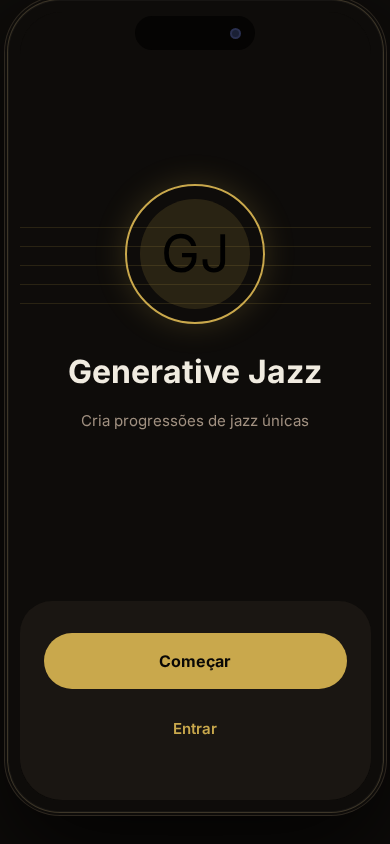
\includegraphics[width=\textwidth]{01_splash.png}
  \caption{Boas-vindas.}
\end{subfigure}\hfill
\begin{subfigure}[t]{0.28\textwidth}
  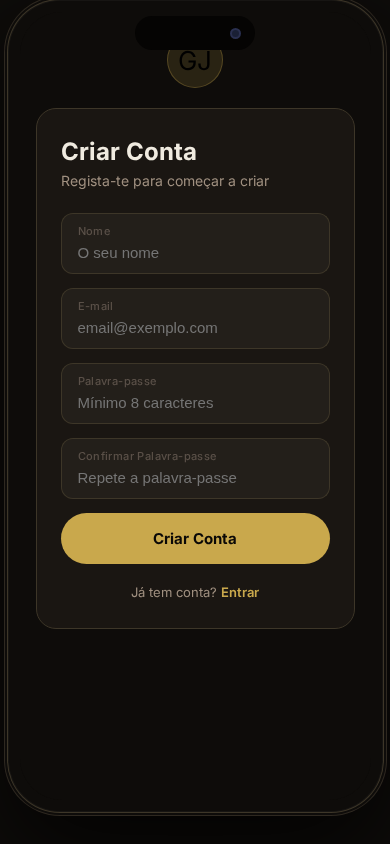
\includegraphics[width=\textwidth]{03_register.png}
  \caption{Registo.}
\end{subfigure}\hfill
\begin{subfigure}[t]{0.28\textwidth}
  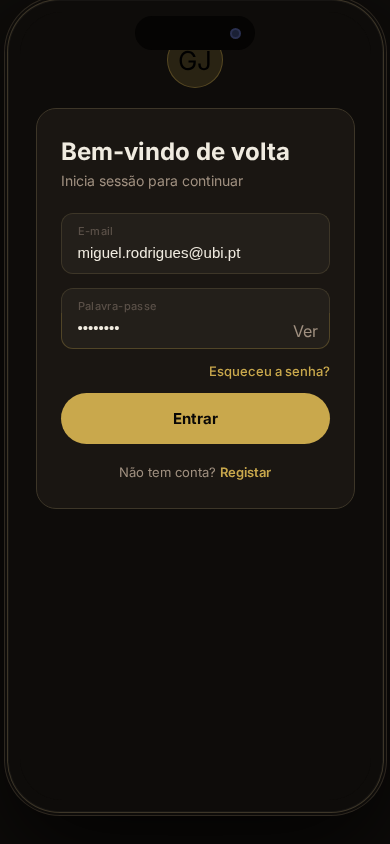
\includegraphics[width=\textwidth]{02_login.png}
  \caption{Login.}
\end{subfigure}
\caption{Ecrãs de acesso à aplicação.}
\label{fig:auth}
\end{figure}

\section{Ecrã Principal e Geração}
\label{chap3:sec:home-geracao}

Depois de entrar, o utilizador chega ao ecrã principal (Figura~\ref{fig:home-gen}a) com uma saudação que muda com a hora do dia, o botão \textbf{Gerar} e as progressões mais recentes. Para criar uma nova, toca-se em \textbf{Gerar} e configuram-se três parâmetros (Figura~\ref{fig:home-gen}b):

\begin{itemize}[noitemsep]
  \item \textbf{Tonalidade} --- selecionada no Círculo das Quintas interativo, ou ``Aleatório'';
  \item \textbf{Estrutura} --- Random, AABA, AABC ou ABAB;
  \item \textbf{Modulação} --- Random, Dominant, Relative, Subdominant, Parallel ou Chromatic.
\end{itemize}

Depois de tocar em \textbf{Gerar Progressão}, uma animação indica que o pedido está a ser processado.

\begin{figure}[!htb]
\centering
\begin{subfigure}[t]{0.28\textwidth}
  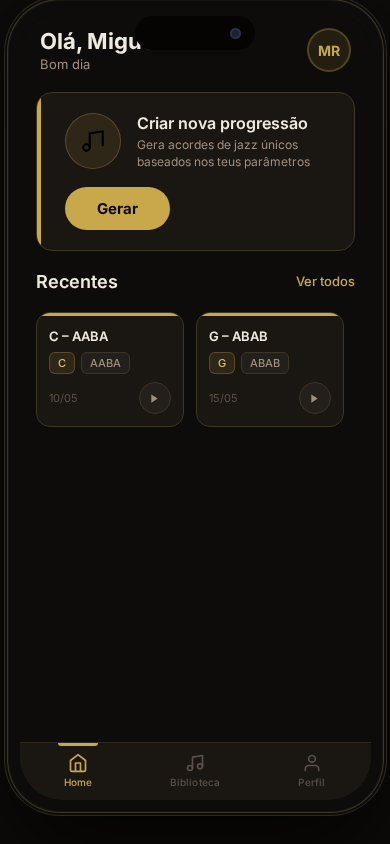
\includegraphics[width=\textwidth]{04_home.png}
  \caption{Ecrã principal.}
\end{subfigure}\hfill
\begin{subfigure}[t]{0.28\textwidth}
  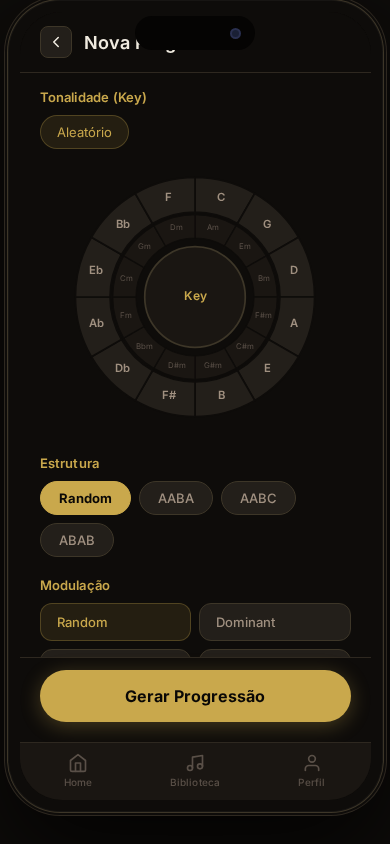
\includegraphics[width=\textwidth]{05_generation.png}
  \caption{Configuração.}
\end{subfigure}\hfill
\begin{subfigure}[t]{0.28\textwidth}
  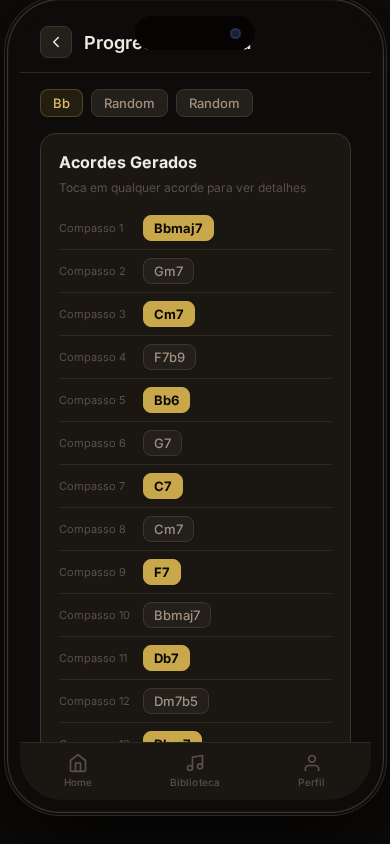
\includegraphics[width=\textwidth]{06_result.png}
  \caption{Resultado.}
\end{subfigure}
\caption{Fluxo principal de geração de uma progressão.}
\label{fig:home-gen}
\end{figure}

\section{Resultado, Biblioteca e Perfil}
\label{chap3:sec:resto}

O ecrã de resultado (Figura~\ref{fig:home-gen}c) mostra a progressão por compassos, um leitor de áudio com play/pausa e barra de progresso, e o cabeçalho com tonalidade, estrutura e modulação. Durante a reprodução o acorde ativo é destacado em tempo real. Para guardar basta tocar em \textbf{Guardar}, editar o nome se necessário, e confirmar.

\begin{figure}[!htb]
\centering
\begin{subfigure}[t]{0.28\textwidth}
  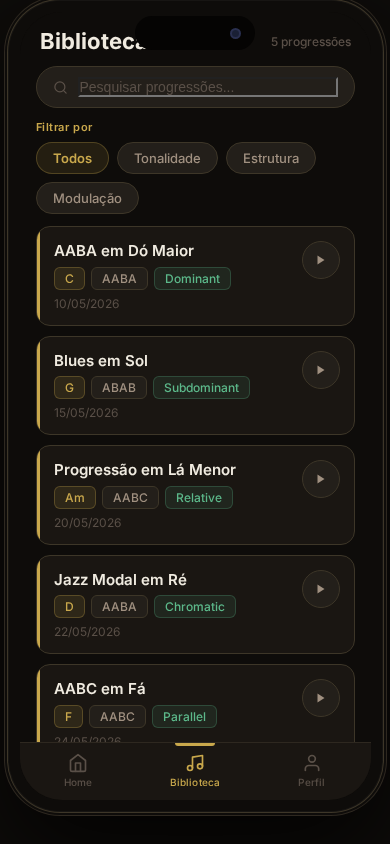
\includegraphics[width=\textwidth]{07_library.png}
  \caption{Biblioteca.}
\end{subfigure}\hfill
\begin{subfigure}[t]{0.28\textwidth}
  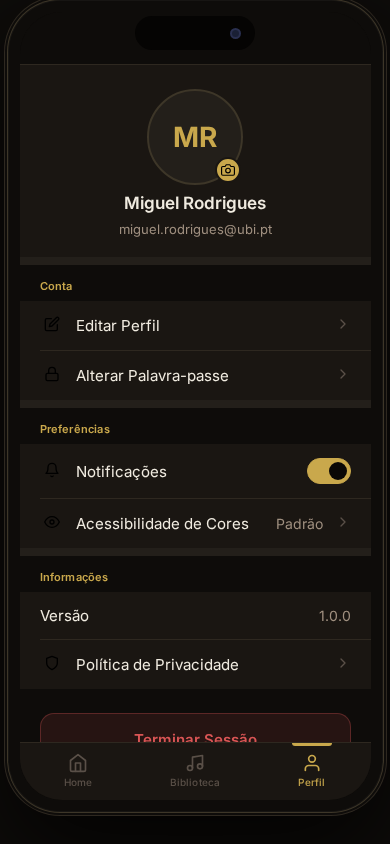
\includegraphics[width=\textwidth]{08_profile.png}
  \caption{Perfil.}
\end{subfigure}\hfill
\begin{subfigure}[t]{0.28\textwidth}
  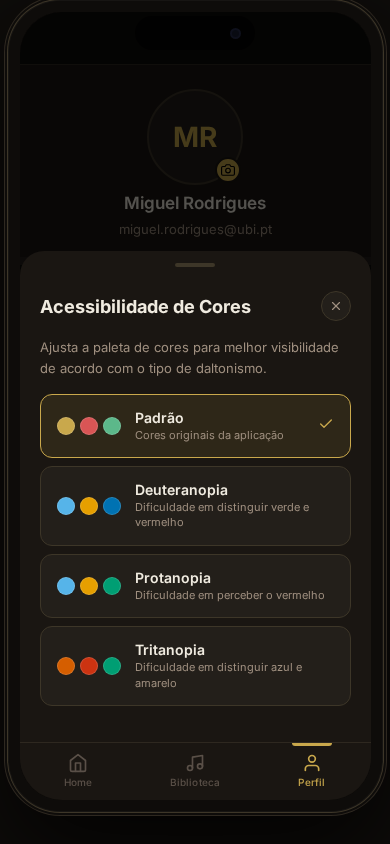
\includegraphics[width=\textwidth]{09_colorblind_sheet.png}
  \caption{Acessibilidade.}
\end{subfigure}
\caption{Biblioteca, perfil e painel de acessibilidade cromática.}
\label{fig:lib-profile}
\end{figure}

A \textbf{Biblioteca} (Figura~\ref{fig:lib-profile}a) lista todas as progressões guardadas com pesquisa em tempo real e reprodução rápida em cada item. O \textbf{Perfil} (Figura~\ref{fig:lib-profile}b) permite editar nome e foto, alterar a palavra-passe, configurar os modos de acessibilidade cromática (Figura~\ref{fig:lib-profile}c) e consultar a política de privacidade. A navegação entre ecrãs autenticados é feita pela barra inferior com ícones de casa, nota musical e utilizador.

\clearpage
\chapter{Decisões de Design e Acessibilidade}
\label{chap:design}

\section{Paleta de Cores}
\label{chap4:sec:cores}

A interface usa um tema escuro com um acento dourado/âmbar. Não foi uma escolha por moda --- cada cor tem uma razão de ser.

O fundo usa \texttt{\#0e0c0a}, um preto com subtom castanho-quente em vez do preto puro. Em ecrãs OLED, o contraste extremo entre fundo preto e texto branco pode ser desconfortável em sessões longas; o subtom quente atenua isso. Visualmente também remete para o ambiente de um clube de jazz, com iluminação ténue, o que se enquadra bem no tema da aplicação.

O acento dourado (\texttt{\#c9a84c}) é a cor de todos os elementos interativos. A associação é direta: saxofone, trompete, trombone --- os instrumentos centrais do jazz têm exatamente esta cor de latão. Além disso o dourado sobre fundo escuro cumpre os rácios de contraste do \ac{WCAG}~2.1 nível AA~\cite{wcag21}, o que não é coincidência. O texto principal usa \texttt{\#f0ebe0}, um branco ligeiramente creme, e o secundário \texttt{\#a09080}. Ambos mantêm a coerência quente da paleta e criam hierarquia clara sem precisar de tamanhos de letra muito diferentes.

Para estados de erro e sucesso escolhemos deliberadamente um vermelho suave (\texttt{\#d95555}) e um verde-azulado (\texttt{\#5cb88a}) em vez de verde puro. A razão é simples: verde e vermelho são as cores mais problemáticas para pessoas com daltonismo, e o verde-azulado já cria distância percetiva suficiente para reduzir confusões mesmo sem ativar nenhum modo de acessibilidade.

\section{Tipografia}
\label{chap4:sec:tipografia}

Usámos exclusivamente a família \textbf{Inter} em pesos de 300 a 700. O protótipo da Parte~1 combinava Playfair Display nos títulos com Inter no corpo, mas abandonámos essa combinação por três razões práticas.

Primeiro, as serifas da Playfair ficavam com aliasing visível a densidades típicas de smartphones Android. Segundo, dois sistemas tipográficos num espaço compacto criam atrito visual sem benefício real --- a hierarquia que a Playfair pretendia introduzir consegue-se perfeitamente com Inter Bold a um tamanho ligeiramente maior. Terceiro, fontes sans-serif com formas abertas são mais fáceis de ler para utilizadores com dislexia~\cite{bda2023}, e a Inter foi desenhada especificamente para interfaces digitais, com aberturas largas nos caracteres e altura-x elevada.

\begin{table}[!htb]
\centering\small
\begin{tabular}{llll}
\toprule
\textbf{Elemento} & \textbf{Peso} & \textbf{Tamanho} & \textbf{Uso} \\
\midrule
Títulos de ecrã   & 700 Bold     & 20--22 px & Cabeçalho de cada ecrã \\
Títulos de secção & 600 SemiBold & 17--18 px & Títulos de cards e painéis \\
Corpo             & 400 Regular  & 14--15 px & Texto corrido \\
Labels            & 500--600     & 11--13 px & Categorias, metadados \\
Texto secundário  & 300--400     & 11--13 px & Datas, dicas \\
\bottomrule
\end{tabular}
\caption{Hierarquia tipográfica Inter na interface do GenJazz.}
\label{tab:tipografia}
\end{table}

\section{Acessibilidade para Utilizadores com Daltonismo}
\label{chap4:sec:daltonismo}

A aplicação inclui três modos de acessibilidade cromática, acessíveis nas definições do perfil. As paletas foram baseadas na paleta de Wong~(2011)~\cite{wong2011}, desenvolvida para garantir discriminabilidade nos principais tipos de deficiência de visão cromática. Cada modo substitui apenas as variáveis CSS de acento, erro e sucesso --- os fundos e textos mantêm-se inalterados.

\begin{table}[!htb]
\centering\small
\begin{tabular}{lp{3.2cm}p{3.2cm}p{3.2cm}}
\toprule
\textbf{Papel} & \textbf{Deuteranopia} & \textbf{Protanopia} & \textbf{Tritanopia} \\
\midrule
Acento  & \texttt{\#56B4E9} azul céu    & \texttt{\#56B4E9} azul céu    & \texttt{\#D55E00} vermelhão \\
Erro    & \texttt{\#E69F00} laranja      & \texttt{\#E69F00} laranja      & \texttt{\#CC3311} verm.-laranja \\
Sucesso & \texttt{\#0072B2} azul escuro  & \texttt{\#009E73} verde-azulado & \texttt{\#009E73} verde-azulado \\
\bottomrule
\end{tabular}
\caption{Paletas de acessibilidade para os três tipos de daltonismo suportados.}
\label{tab:daltonismo}
\end{table}

A deuteranopia --- dificuldade em perceber o verde, presente em cerca de 5--6\% da população masculina~\cite{birch2012} --- foi o caso que mais justificou esta funcionalidade, uma vez que o dourado da paleta padrão tem uma componente verde que o torna difícil de distinguir neste modo de visão. Para a protanopia (ausência de sensibilidade ao vermelho, \textasciitilde1\%) a paleta é parecida mas com o sucesso ajustado, pois protanopes conseguem distinguir verdes deslocados para o ciano. Para a tritanopia (afeta o azul, \textasciitilde0,01\%) o dourado é substituído por vermelhão, que não depende da distinção azul/amarelo.

\begin{figure}[!htb]
\centering
\begin{subfigure}[t]{0.28\textwidth}
  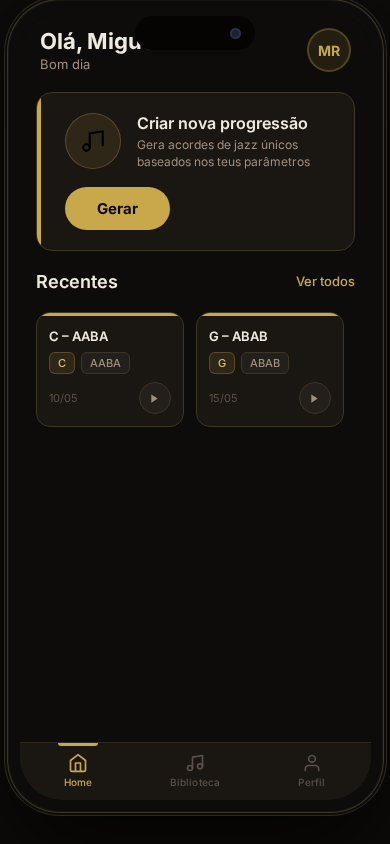
\includegraphics[width=\textwidth]{04_home.png}
  \caption{Padrão.}
\end{subfigure}\hfill
\begin{subfigure}[t]{0.28\textwidth}
  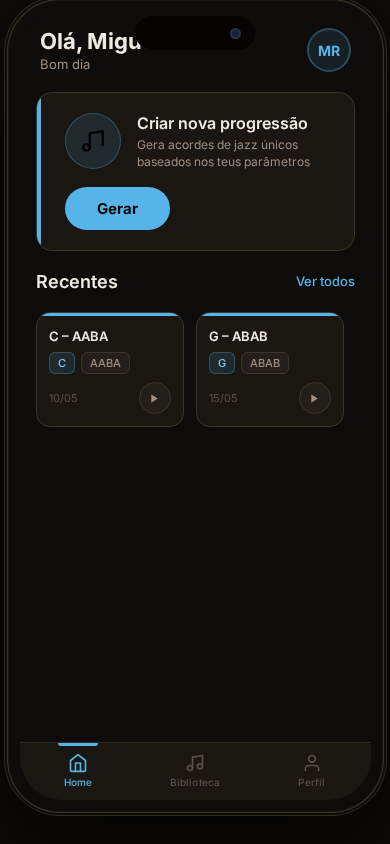
\includegraphics[width=\textwidth]{11_home_deuteranopia.png}
  \caption{Deuteranopia.}
\end{subfigure}\hfill
\begin{subfigure}[t]{0.28\textwidth}
  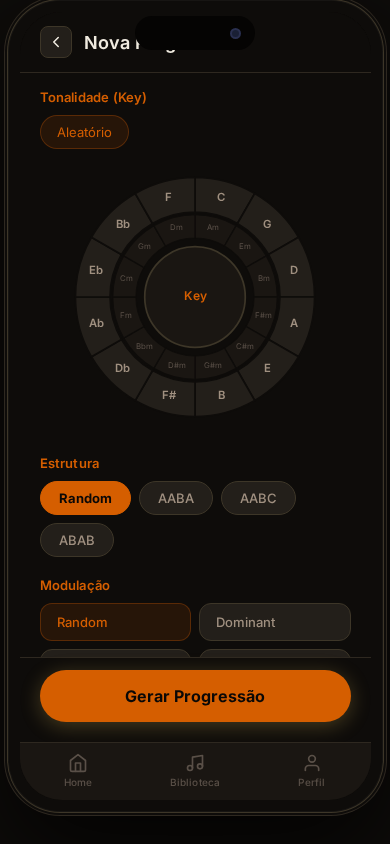
\includegraphics[width=\textwidth]{12_generation_tritanopia.png}
  \caption{Tritanopia.}
\end{subfigure}
\caption{Comparação entre o modo padrão e dois modos de acessibilidade cromática.}
\label{fig:daltonismo}
\end{figure}

A implementação é feita exclusivamente via variáveis CSS: ao mudar o modo, adiciona-se o atributo \texttt{data-colorblind} ao elemento \texttt{<html>} e as variáveis corretas são automaticamente aplicadas em toda a interface, sem alterar nenhum componente individualmente.

\section{Outras Considerações de Acessibilidade}
\label{chap4:sec:outras}

Para além dos modos de daltonismo, tomámos algumas decisões que melhoram a acessibilidade geral. Todos os pares de cor texto/fundo foram verificados para cumprir o nível AA do \ac{WCAG}~2.1. Os botões e elementos tácteis têm pelo menos 44$\times$44~px, seguindo as recomendações da Apple e do W3C. A hierarquia da interface é transmitida por tamanho, peso e posição, não dependendo só de cor --- o que faz com que a interface funcione bem mesmo no modo de alto contraste do sistema operativo.

\clearpage
\chapter{Alterações ao Protótipo da 1.\textsuperscript{a} Parte}
\label{chap:alteracoes}

Ao passar do protótipo para a implementação real surgiram três situações em que foi necessário ajustar ou acrescentar funcionalidades. Esta secção descreve o que mudou e porquê.

\section{Acessibilidade Cromática}
\label{chap5:sec:alt1}

A funcionalidade de modos de daltonismo não estava prevista no protótipo original. A necessidade tornou-se óbvia quando percebemos que o dourado da paleta padrão tem uma componente de verde que cria problemas para utilizadores com deuteranopia --- o tipo de daltonismo mais comum, que afeta cerca de 5--6\% da população masculina~\cite{birch2012}. Ignorar este problema seria uma barreira de exclusão desnecessária.

A solução foi adicionar três modos alternativos no perfil, cada um com uma paleta baseada nos trabalhos de Wong~(2011)~\cite{wong2011}. O painel de seleção mostra uma pré-visualização das três cores principais antes de o utilizador confirmar, para que possa ver o efeito sem ter de andar a mudar às cegas. A alteração responde diretamente à Heurística~7 de Nielsen --- flexibilidade e eficiência --- que preconiza que a interface se adapte a diferentes perfis de utilizadores~\cite{nielsen1994}.

\section{Política de Privacidade}
\label{chap5:sec:alt2}

Outra adição não prevista foi a secção de Política de Privacidade no perfil. O \ac{RGPD} exige que os utilizadores sejam informados sobre o tratamento dos seus dados mesmo em contexto académico, e mesmo quando tudo fica guardado localmente. Mas há também uma razão de \ac{UX}: um utilizador que não sabe o que acontece com os seus dados tende a usar a aplicação com desconfiança. A política é curta e direta --- explica o âmbito educacional da aplicação, o que a API recebe, e como apagar os dados locais --- e isso é suficiente para gerir as expectativas de forma honesta.

\section{Tipografia --- Remoção da Playfair Display}
\label{chap5:sec:alt3}

O protótipo usava Playfair Display nos títulos e Inter no corpo. Na implementação passámos a usar apenas Inter em toda a interface. O motivo foi essencialmente prático: ao renderizar em ecrãs de densidade intermédia, as serifas da Playfair tinham aliasing visível que tornava os títulos menos nítidos do que o texto em Inter. Além disso, manter duas famílias tipográficas num ecrã pequeno criava um atrito visual que não justificava qualquer benefício real --- a hierarquia ficou igualmente clara usando apenas pesos diferentes da Inter.

\clearpage
\chapter{Conclusões e Trabalho Futuro}
\label{chap:conc-trab-futuro}

\section{Conclusões}
\label{sec:conc-princ}

O GenJazz cumpriu o objetivo principal desta fase: transformar o protótipo em algo que funciona de verdade, fiel ao conceito original mas com os ajustes que só a implementação real consegue revelar. O fluxo central --- gerar uma progressão, ouvi-la e guardá-la --- é rápido e direto, com poucos passos entre o utilizador e o resultado. A arquitetura \textit{local-first} funcionou bem na prática: a interface responde de imediato sem depender da latência da rede para operações básicas.

Do ponto de vista de \ac{IHC}, a funcionalidade de acessibilidade cromática foi provavelmente a contribuição mais significativa desta fase. Não estava prevista no protótipo e surgiu durante a implementação quando percebemos que a paleta padrão excluía uma parte dos utilizadores sem qualquer necessidade. Resolver isso com paletas baseadas em investigação publicada e uma implementação via variáveis CSS globais foi uma escolha que valeu a pena.

\section{O Que Não Foi Implementado}
\label{sec:nao-implementado}

Algumas funcionalidades esboçadas na Parte~1 não chegaram a esta versão. A \textbf{sincronização de conta entre dispositivos} implicaria um servidor de autenticação próprio que está fora do âmbito deste projeto --- a API pública do GenJazz não tem suporte para autenticação de utilizadores. O \textbf{modo offline completo com cache de áudio} exigiria um Service Worker com estratégia de cache de ficheiros MP3, o que não foi desenvolvido por falta de tempo. A \textbf{exportação de partituras} dependeria de uma biblioteca de renderização musical (como VexFlow) cuja integração teria ultrapassado o âmbito da \ac{IHC}.

\section{Trabalho Futuro}
\label{sec:trab-futuro}

As três funcionalidades não implementadas são os candidatos mais naturais para uma versão futura. Para além destas, seria útil fazer uma sessão de testes de usabilidade com utilizadores reais --- a avaliação interna tem limites óbvios. Adicionar atributos ARIA adequados para suporte a leitores de ecrã seria também um passo importante para tornar a aplicação verdadeiramente inclusiva.

\clearpage

\appendix
\chapter{Declaração de Utilização de Inteligência Artificial}
\label{chap:ai-disclaimer}

No desenvolvimento deste projeto recorremos pontualmente a ferramentas de \ac{IA} generativa em situações específicas.

As ferramentas foram usadas principalmente na \textbf{escolha de cores e tipografia}: quando tínhamos dúvidas sobre combinações de cor, rácios de contraste ou sobre qual a fonte mais adequada para determinados contextos de interface, usámos assistentes de \ac{IA} para discutir opções e obter referências adicionais. O mesmo se aplicou a \textbf{dúvidas estéticas e de propriedades de utilização} ao longo do desenvolvimento --- questões sobre espaçamento, hierarquia visual, dimensionamento de elementos tácteis e similares. Foram também usadas para \textbf{correção de bugs e erros} que foram surgindo durante o desenvolvimento, como problemas de renderização em determinados browsers ou comportamentos inesperados de componentes React.

As decisões finais --- tanto de design como de implementação --- foram sempre tomadas pelo grupo. 
As ferramentas utilizadas foram o \textbf{Claude} e o \textbf{Gemini}.

\clearpage

\backmatter

\end{document}
